% 
% Lecture Template for ME3023 -  Measurements in Mechanical Systems - Tennessee Technological University
%
% Spring 2020 - Summer 2020
% Tristan Hill, May 07, 2020 - June 12, 2020
% Module 5 - Strain Applications
% Topic 3 - Principle Strains
%

%\documentclass{beamer}                         % for presentation (has nav buttons at bottom)
\documentclass[handout]{beamer}  % for handout 
\usepackage{beamerthemesplit}
\usepackage{amsmath}
\usepackage{listings}
\usepackage{multicol}
\usepackage{framed}

\beamertemplateballitem

% custom colors
\definecolor{TTUpurple}{rgb}{0.3098, 0.1607, 0.5176} % TTU Purple (primary)
\definecolor{TTUgold}{rgb}{1.0000, 0.8666, 0.0000} % TTU Gold (primary) 
\definecolor{mygray}{rgb}{.6, .6, .6}
\definecolor{mypurple}{rgb}{0.6,0.1961,0.8}
\definecolor{mybrown}{rgb}{0.5451,0.2706,0.0745}
\definecolor{mygreen}{rgb}{0, .39, 0}
\definecolor{mypink}{rgb}{0.9960, 0, 0.9960}

% color commands
\newcommand{\R}{\color{red}}
\newcommand{\B}{\color{blue}}
\newcommand{\BR}{\color{mybrown}}
\newcommand{\K}{\color{black}}
\newcommand{\G}{\color{mygreen}}
\newcommand{\PR}{\color{mypurple}}
\newcommand{\PN}{\color{mypink}}
\newcommand{\OR}{\color{TTU}}
\newcommand{\GD}{\color{TTUgold}}


\setbeamercolor{palette primary}{bg=TTUpurple,fg=TTUgold}
\setbeamercolor{palette secondary}{bg=black,fg=TTUgold}
\setbeamercolor{palette tertiary}{bg=black,fg=TTUpurple}
\setbeamercolor{palette quaternary}{bg=TTUgold,fg=black}
\setbeamercolor{structure}{fg=TTUpurple} % itemize, enumerate, etc
\setbeamercolor{section in toc}{fg=TTUpurple} % TOC sections

%\usefonttheme{professionalfonts}

\newcommand{\Lagr}{\mathcal{L}} % lagrangian

\newcommand{\hspcu}{\underline{\hspace{20mm}}} % large horizontal space w underline
\newcommand{\vspccc}{\vspace{6mm}\\} % large vertical space
\newcommand{\vspcc}{\vspace{4mm}\\}   % medium vertical space
\newcommand{\vspc}{\vspace{2mm}\\}     % small vertical space

\newcommand{\hspcccc}{\hspace{10mm}} % large horizontal space
\newcommand{\hspccc}{\hspace{6mm}} % large horizontal space
\newcommand{\hspcc}{\hspace{4mm}}   % medium horizontal space
\newcommand{\hspc}{\hspace{2mm}}     % small horizontal space

\newcommand{\eqscl}{0. 9}     % small horizontal space


\author{ME3023 - Measurements in Mechanical Systems} % original formatting from Mike Renfro, September 21, 2004

\newcommand{\MNUM}{5\hspace{2mm}} % Module number
\newcommand{\TNUM}{3\hspace{2mm}} % Topic number 
\newcommand{\moduletitle}{Strain Applications}
\newcommand{\topictitle}{Principle Strains} 

\newcommand{\sectiontitleI}{Motivation}
\newcommand{\sectiontitleII}{Principle Stress and Strain}
\newcommand{\sectiontitleIII}{Determining Principle Stresses}
\newcommand{\sectiontitleIV}{Example: A Pressure Vessel}

% custom box
\newsavebox{\mybox}

\title{Module \MNUM - \moduletitle}

\date{Mechanical Engineering\vspc Tennessee Technological University}

\begin{document}

\lstset{language=MATLAB,basicstyle=\ttfamily\small,showstringspaces=false}

\frame{\titlepage \center\begin{framed}\Large \textbf{Topic \TNUM - \topictitle}\end{framed} \vspace{5mm}}

% Section 0: Outline
\frame{

\large \textbf{Topic \TNUM - \topictitle} \vspace{3mm}\\

\begin{itemize}

	\item \sectiontitleI		\vspc % Section I
	\item \sectiontitleII 	\vspc % Section II
	\item \sectiontitleIII 	\vspc %Section III
	\item \sectiontitleIV 	\vspc %Section IV

\end{itemize}

}

% Section I:
\section{\sectiontitleI}

% Section I - Frame I:
\frame{
\frametitle{\sectiontitleI}

The design of load-carrying components for machines and structures requires information concerning the {\B distribution of forces within the particular component}. Proper design of devices such as shafts, pressure vessels, and support structures must consider {\PR load-carrying capacity and allowable deflections}. Mechanics of materials provides a basis for predicting these essential characteristics of a mechanical design, and provides the fundamental understanding of the behavior of load-carrying parts. However, theoretical analysis is often not sufficient, and {\PN experimental measurements} are required to achieve a final design.

{\tiny Text: Theory and Design of Mechanical Measurements}
}


% Section II:
\section{\sectiontitleII}

% Section II - Frame I:
\frame{
\frametitle{\sectiontitleII}

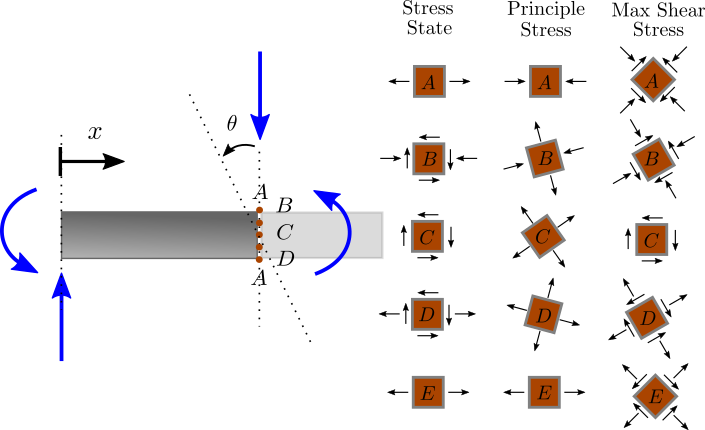
\includegraphics[scale=.5]{stress_states.png}


}

% Section II - Frame II:
\frame{
\frametitle{\sectiontitleII}


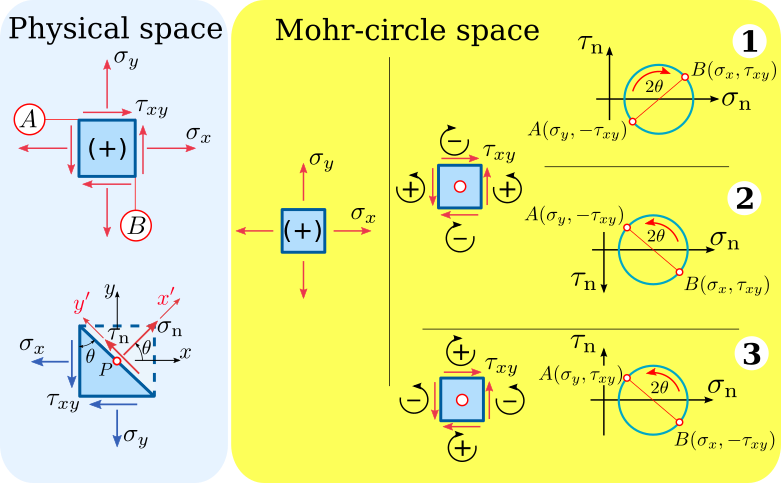
\includegraphics[scale=.45]{mohrs_circle.png}\\
{\tiny Image: \href{https://en.wikipedia.org/wiki/Mohr\%27s_circle}{Wikipedia}}
}


% Section III:
\section{\sectiontitleIII}

% Section III - Frame I:
\frame{
\frametitle{\sectiontitleIII}

A strain gauge rosette can be mounted on a physical component to measure the principle strains and their directions. Depending on what is known about the stress state this may be done in one of four ways.

\begin{itemize}
\item Case 1: Uniaxial Stress \vspc
\item Case 2: Isotropic Stress \vspc
\item Case 3: Pure Torsional Stress \vspc
\item Case 4: Biaxial Stress 
	\begin{itemize}
		\item with known principle directions 
		\item or with unknown principle directions 
	\end{itemize}
\end{itemize}

\vspace{20mm}
{\tiny Text: Theory and Design of Mechanical Measurements}
}

% Section III - Frame II:
\frame{
\frametitle{\sectiontitleIII}
\begin{multicols}{2}
\underline{Case 1: Uniaxial Stress} 
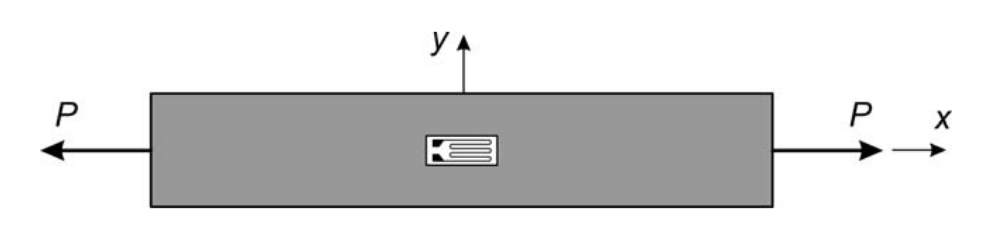
\includegraphics[scale=.18]{metu_fig1.png} \vspc
\underline{Case 2: Isotropic Stress} 
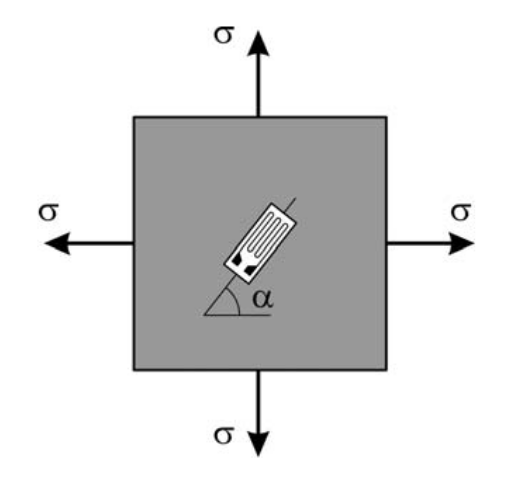
\includegraphics[scale=.18]{metu_fig2.png}

\scalebox{1}{$\sigma_{xx}=E\epsilon_{xx}$} \vspace{25mm}\\

\scalebox{1}{$\sigma_{xx}=\sigma_{yy}=\sigma_1=\sigma_2=\sigma=\frac{E\nu}{1-\nu}$}\vspc
\scalebox{1}{$\tau_{xy}=0$}\vspc


\end{multicols}

\vspace{20mm}
{\tiny Text: Theory and Design of Mechanical Measurements}
}

% Section III - Frame III:
\frame{
\frametitle{\sectiontitleIII}

\underline{Case 3: Pure Torsional Stress} 
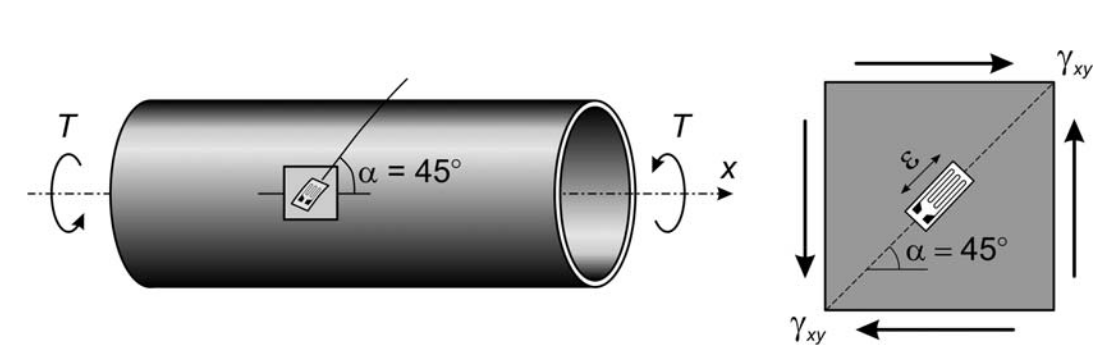
\includegraphics[scale=.18]{metu_fig3.png}

\scalebox{1}{$\tau_{xy}=\tau_{max}=G\gamma_{xy}$ \hspc with\hspc $\gamma=2\epsilon$}\vspc

\underline{Case 4a: Biaxial Stress} - The principle directions are known.\vspc
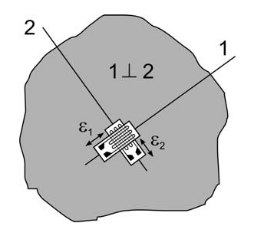
\includegraphics[scale=.20]{metu_fig4.png}

\scalebox{1}{$\sigma_1=\frac{E}{1-\nu^2}\left(\epsilon_1+\nu\epsilon_2\right)$ \hspc and \hspc $\sigma_2=\frac{E}{1-\nu^2}\left(\epsilon_2+\nu\epsilon_1\right)$}\vspc

}

% Section III - Frame IV:
\frame{
\frametitle{\sectiontitleIII}

\underline{Case 4b: Biaxial Stress} - The principle directions are not known.\vspc
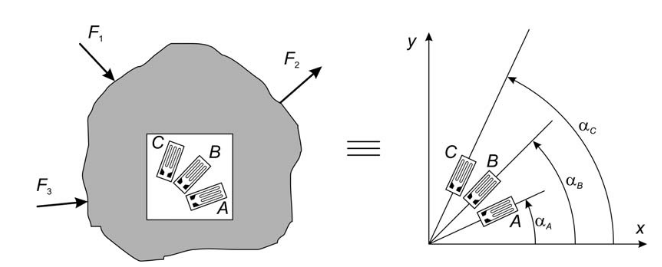
\includegraphics[scale=.25]{metu_fig5.png}
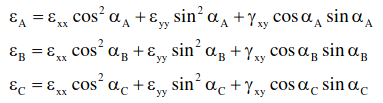
\includegraphics[scale=.3]{metu_fig8.png}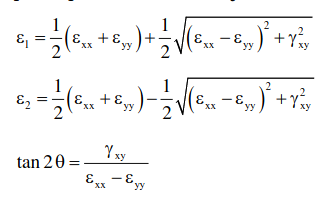
\includegraphics[scale=.3]{metu_fig9.png}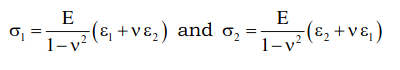
\includegraphics[scale=.3]{metu_fig10.png}


\vspace{20mm}
{\tiny Text: }
}


% Section IV:
\section{\sectiontitleIV}

% Section IV - Frame I:
\frame{
\frametitle{\sectiontitleIV}

A practical example of this can be seen \href{http://cecs.wright.edu/~rsrin/Courses/Egr190-191/PV-EGR191.pdf}{\PR here} in which a strain gauge is used to measure the pressure in a tank from a strain reading alone. \vspc

Which case from above are do they use?

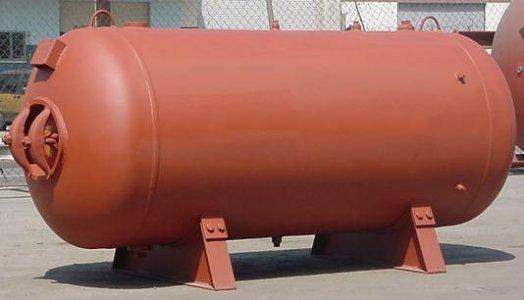
\includegraphics[scale=.4]{pressure_vessel.jpg}

}
	
\end{document}





